

\subsection{Determining the cutoff between expansions}

With these error bounds in hand, we precompute the following tables for
tolerances $\epsilon = \texttt{1e-4}, \dots, \texttt{1e-15}$, orders $\nu = 1,
\dots, 100$, and number of asymptotic expansion terms $M = 1, \dots, 20$
\begin{list}{$\circ$}{}
    \item $z_{\nu, \epsilon}^M$ such that the $M$-term asymptotic expansion of
    $J_\nu(\omega r)$ is $\epsilon$-accurate for all $\omega r > z_{\nu,
    \epsilon}^M$
    \item $L_{\nu, \epsilon}^M$ such that the $L_{\nu, \epsilon}^M$-term Wimp
    expansion of $J_\nu(\omega r)$ is $\epsilon$-accurate for all $\omega r \leq
    z_{\nu, \epsilon}^M$
\end{list}
Therefore, for any order $\nu$ we can look up a pair of complementary local and
asymptotic expansions with error everywhere bounded by the requested tolerance
$\epsilon$. The only remaining free parameter is the number of asymptotic terms
$M$. This parameter is selected heuristically in our implementation as 
\begin{align} \label{eq:num-asy-terms}
    M = \min\left(\flr{1 + \frac{\nu}{5} - \frac{\log_{10}(\epsilon)}{4}}, 20\right)
\end{align}
according to numerical experiments which maximize speed by balancing the cost of
the local, asymptotic, and direct evaluations.

\subsection{Subdividing the matrix into blocks by expansion}

Having established error bounds which allow us to automatically select the
number of asymptotic terms $M$, local terms $L$, and crossover point $z$ given a
tolerance $\epsilon$ and order $\nu$, we now discuss how to subdivide the matrix
$\bm{A}$ into three sets of blocks, each of which can be efficiently applied to
a vector as described above:
\begin{list}{$\circ$}{}
    \item Local blocks $\mathscr{L} = \big\{ (j_0:j_1, k_0:k_1) \ | \ \omega_j
    r_k \leq z \ \forall \ j_0 \leq j \leq j_1, \ k_0 \leq k \leq k_1 \big\}$
    \item Asymptotic blocks $\mathscr{A} = \big\{ (j_0:j_1, k_0:k_1) \ | \
    \omega_j r_k > z \ \forall \ j_0 \leq j \leq j_1, \ k_0 \leq k \leq k_1
    \big\}$
    \item Direct blocks $\mathscr{D}$ which are small enough that no fast
    expansion is needed
\end{list}
In order to determine a subdivision of $\bm{A}$ into blocks of these three
types, we initialize a set of \textit{mixed} blocks $\mathscr{M} = \{(1:m,
1:n)\}$, which contains a mix of local and asymptotic entries. We then chose an
index pair $(j,k)$ such that $\omega_j r_k \approx z$. This index subdivides the
block into four new sub-blocks with $(j,k)$ at the center, so that the upper
left block can be applied using the local expansion and is appended to
$\mathscr{L}$, the lower right block using the asymptotic expansion and is
appended to $\mathscr{A}$. 

The remaining lower left and upper right blocks each still contain a mix of
local and asymptotic entries. If they are of sufficiently small size $m_b \times
n_b$ with $m_b n_b < \texttt{min\_size} := 1024$, they can be evaluated directly
and are appended to $\mathscr{D}$. Otherwise they are appended back to
$\mathscr{M}$, and we continue the subdivision process recursively. 

This method yields a valid partition for any choice of $(j,k)$, but for
efficiency these indices are chosen to maximize the number of matrix entries
which can be applied using a fast expansion, i.e. the sizes of the upper left
and lower right blocks. This is done by solving the following constrained
optimization problem
\begin{align}
    (j,k) 
    &\ = \textsc{SplitIndices}(r_1,\dots,r_n, \omega_1,\dots,\omega_m, z) \\
    &:= \left\{
        \begin{array}{r@{\quad } l}
        \text{argmax} & (j-j_0)(k_1-k) + (j_1-j)(k-k_0)   \\
        \text{subject to} & j_0 \leq j \leq j_1 \\ 
        & k_0 \leq k \leq k_1 \\ 
        & \omega_j r_k \leq z
        \end{array}
    \right. \label{eq:subdiv-optim}
\end{align}
This problem can be solved exactly in \red{$\bO(j_1 - j_0 + k_1 - k_0)$?} time
using \red{bisection?}. However, computing the exact optimal splitting indices
for every box gives a negligible speedup overall compared to a simpler,
quasi-optimal scheme. In practice it is sufficient to choose a small number of
equispaced indices $j \in j_0:j_1$, compute the corresponding $k = \argmax \{k \
| \ r_k \leq \frac{z}{\omega_j}\}$ for each $j$, and choose $(j,k)$ as the pair
which minimizes the objective function of (\ref{eq:subdiv-optim}) among this
small collection.

\begin{algorithm2e}[t]
    \caption{Block subdivision of Hankel transform
    matrix}\label{alg:subdivision}
    \SetKwFunction{Subdivide}{Subdivide}
\Function{\Subdivide{$\bm{r}, \bm{\omega}, z, \texttt{\upshape min\_size}$}}{
    $\mathscr{L} = \mathscr{A} = \mathscr{D} = \emptyset$ \\
    $\mathscr{M} = \{(1:m, 1:n)\}$ \\
    \While{$\mathscr{M} \neq \emptyset$}{
        Pop an element $(j_0 : j_1, k_0 : k_1)$ from $\mathscr{M}$ \\
        $(j,k) = \textsc{SplitIndices}(r_{j_0},\dots,r_{j_1}, \omega_{k_0},\dots,\omega_{k_1}, z)$ \\
        Append $(j_0:j, k_0:k)$ to $\mathscr{L}$ \\
        Append $(j+1:j_1, k+1:k_1)$ to $\mathscr{A}$ \\
        Append $(j_0:j, k+1:k_1)$ to $\mathscr{M}$ \textbf{if} $(j - j_0 + 1)(k_1 - k) > \texttt{\upshape min\_size}$ \textbf{else} $\mathscr{D}$ \\
        Append $(j+1:j_1, k_0:k)$ to $\mathscr{M}$ \textbf{if} $(j_1 - j)(k_1 - k + 1) > \texttt{\upshape min\_size}$ \textbf{else} $\mathscr{D}$
    }
    \Return{$(\mathscr{L}, \mathscr{A}, \mathscr{D})$}
}
\end{algorithm2e}

\begin{algorithm2e}[t]
    \caption{Nonuniform fast Hankel transform}\label{alg:nufht}
    \SetKwFunction{NUFHT}{NUFHT}
\Function{\NUFHT{$\nu, \epsilon, \bm{r}, \bm{c}, \bm{\omega}$}}{
    $\bm{g} = \bm{0}$ \\
    Choose $M$ using (\ref{eq:num-asy-terms}) \\
    Look up $L = L_{\nu,\epsilon}^{M}$ and $z = z_{\nu,\epsilon}^{M}$ from pre-computed tables \\
    Choose \texttt{\upshape min\_size} from numerical experiments (e.g. default 1024)
    $(\mathscr{L}, \mathscr{A}, \mathscr{D}) = \textsc{Subdivide}(r_1,\dots,r_n, \omega_1,\dots,\omega_m, z, \texttt{\upshape min\_size})$ \\
    \For{$\mathscr{B} \in (\mathscr{L}, \mathscr{A}, \mathscr{D})$}{
        \For{$(j_0:j_1, k_0:k_1) \in \mathscr{B}$}{
            $\bm{g}(j_0:j_1) \pluseq \bm{A}(j_0:j_1, k_0:k_1) \bm{c}(k_0:k_1)$ using corresponding expansion \\
        }
    }
    \Return{$\bm{g}$}
}
\end{algorithm2e}

\begin{figure}
    \centering
    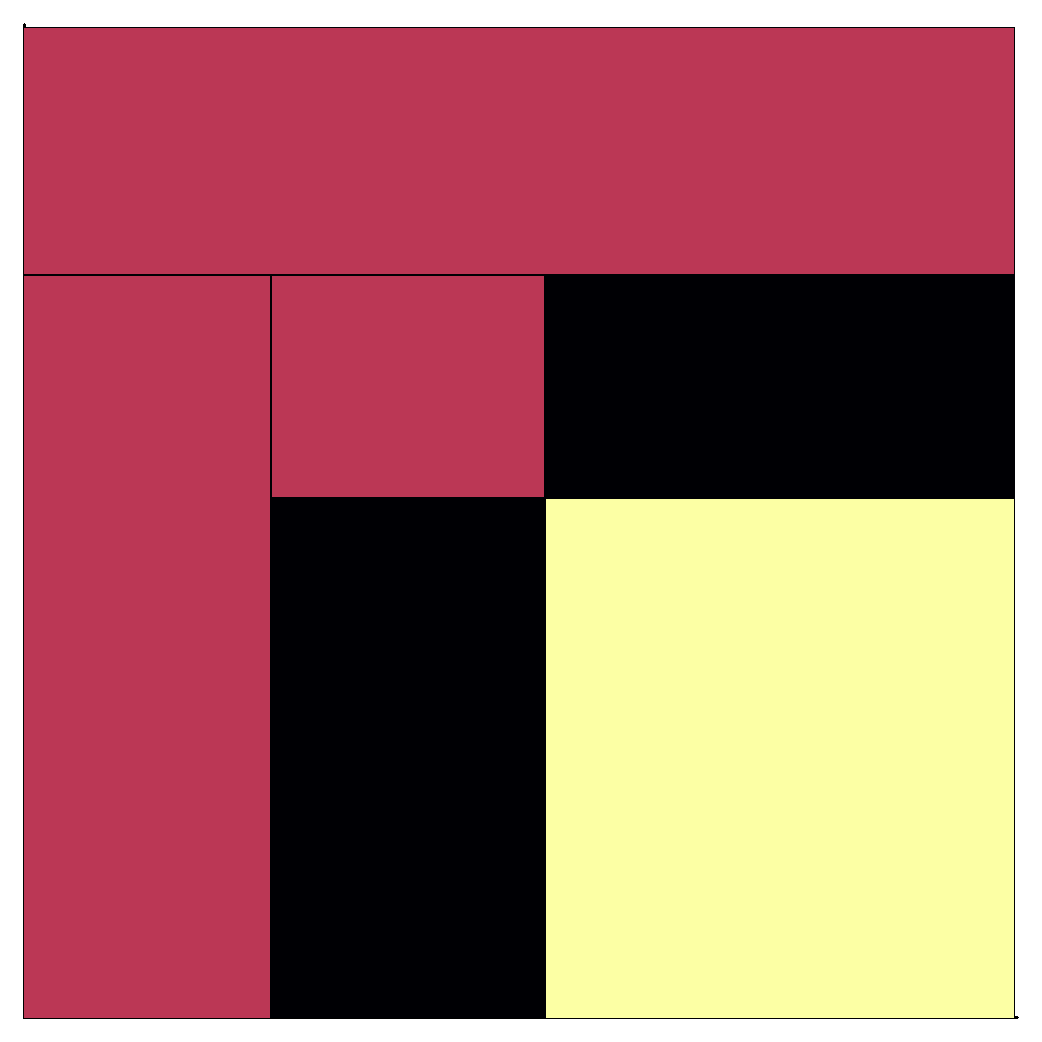
\includegraphics[width=0.23\textwidth]{./figures/nufht_boxes_lvl1.pdf}
    \hfill
    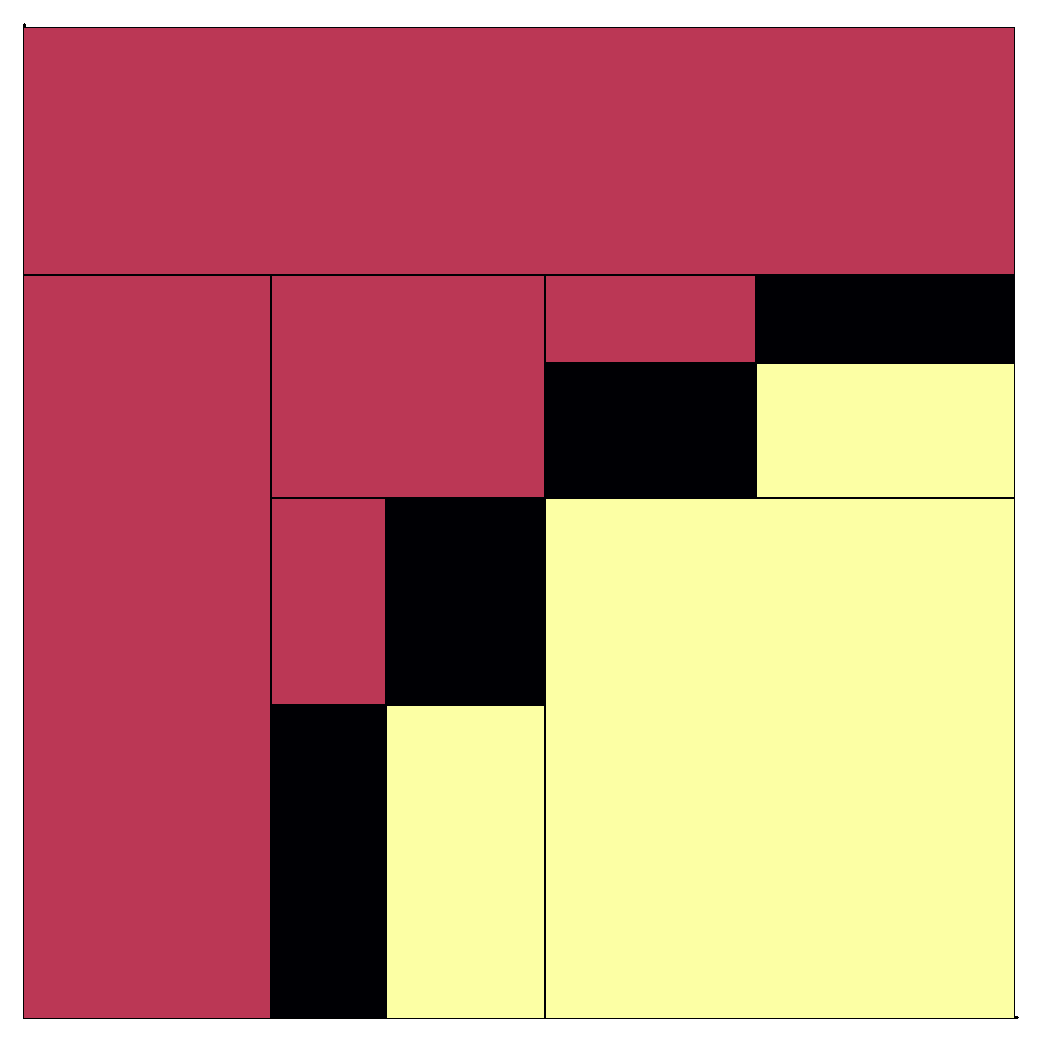
\includegraphics[width=0.23\textwidth]{./figures/nufht_boxes_lvl2.pdf}
    \hfill
    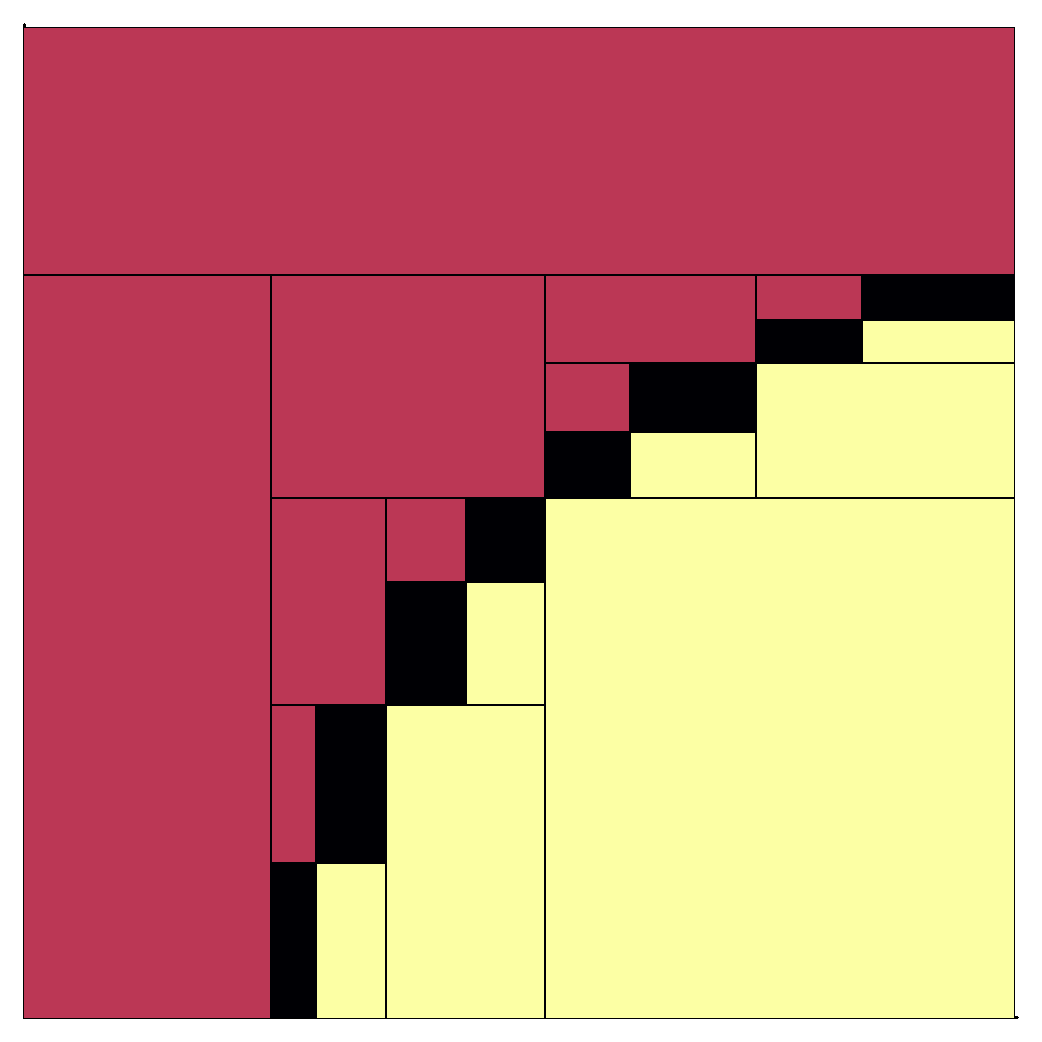
\includegraphics[width=0.23\textwidth]{./figures/nufht_boxes_lvl3.pdf}
    \hfill
    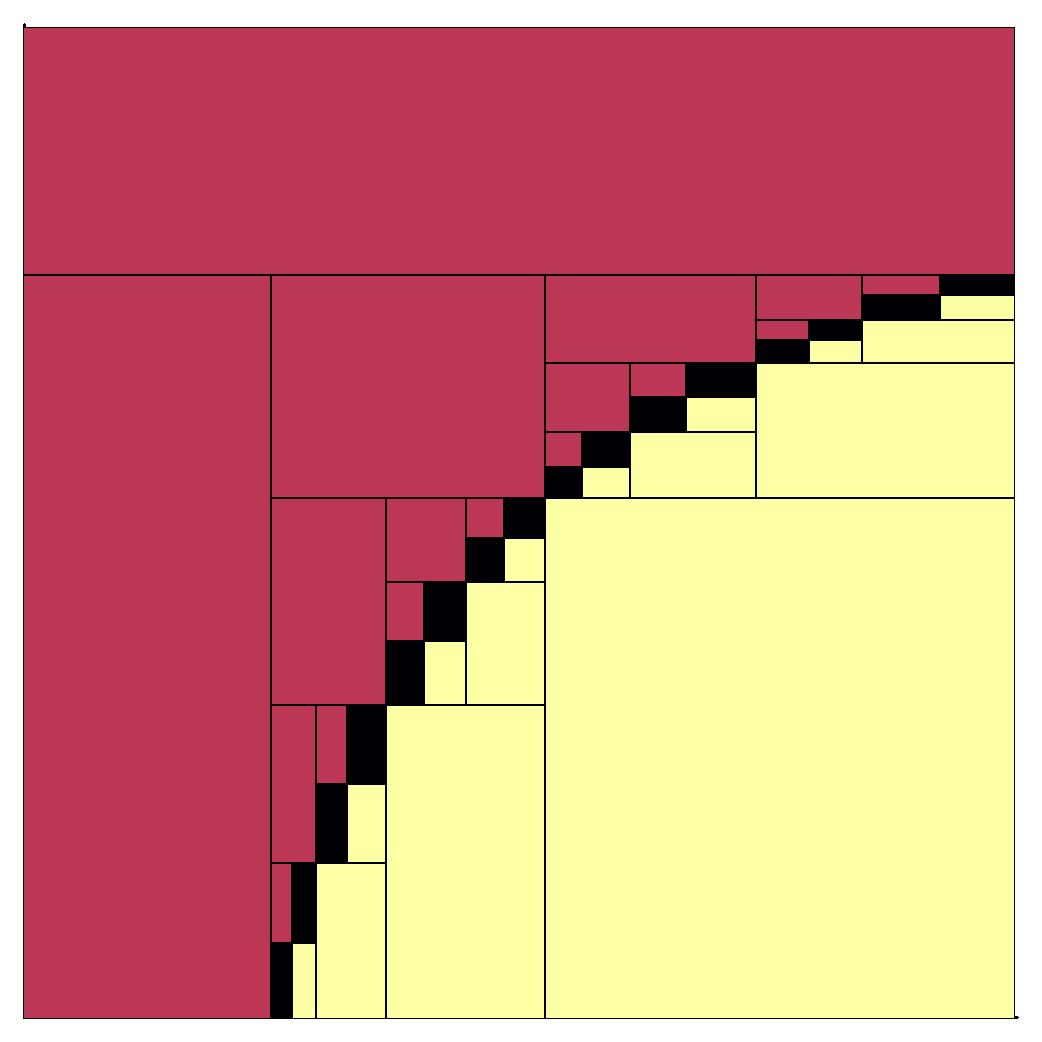
\includegraphics[width=0.23\textwidth]{./figures/nufht_boxes_lvl4.pdf}
    \caption{Direct (black), local (red), and asymptotic (yellow) boxes of
    $J_\nu(\omega_j r_k)$}
\end{figure}

\subsection{Computational complexity}

We now analyze the computational complexity of the proposed approach. In order
to do so, we must first comment on the complexity of the NUFFT, which is an
important subroutine in our method. Nearly all analysis-based NUFFT codes ---
including the FINUFFT library \cite{barnett2019parallel} which we use in our
NUFHT implementation --- consist of three steps. First, delta masses centered at
each non-uniform point are convolved with a \textit{spreading function} which
smears them onto a fine $N$-point uniform grid. Then, a standard equispaced FFT
is computed on the fine grid. Finally, a diagonal de-convolution with the
Fourier transform of the spreading function is applied to reverse the effect of
the original smearing. For a more complete description of the NUFFT, see
\todocite. For $n$ locations $r_k$ and $m$ frequencies $\omega_j$, the dominant
costs in the NUFFT are... \red{explain spreading and FFT costs, why fine grid
size $N$ scales like $\bO(n)$ for type-I, $\bO(m)$ for type-II, and like the
space-frequency product $\bO(\Omega R)$ for type-III.}

\begin{theorem}
    Let $\omega_1,\dots,\omega_m \in [0,1]$ and $r_1,\dots,r_n \in [0,n]$. Then
    the computational cost of computing the NUFHT to tolerance $\epsilon$ using
    Algorithm \ref{alg:nufht} is $\bO\big((m + n\log n) \log \min(n,m) \big)$.
\end{theorem}

\begin{proof}
    If $\omega_j r_k \leq z$ for all $j=1,\dots,n$ and $k=1,\dots,m$ then only
    the low-rank local expansion is used, resulting in $\bO(m + n)$ complexity.
    If instead $\omega_j r_k > z$ everywhere, then only the asymptotic expansion
    is used, giving $\bO(m + n\log n)$ complexity.

    Otherwise, consider the case where $\bm{A}$ contains both local and
    asymptotic entries. After step $\ell$ of subdividing every mixed block, we
    obtain $2^{\ell}$ new mixed blocks, $2^{\ell-1}$ new local blocks, and
    $2^{\ell-1}$ new asymptotic blocks. Let the local blocks be of size
    $m_{\ell,b} \times n_{\ell,b}$ for $b = 1,\dots,2^{\ell-1}$. Then
    $\sum_{b=1}^{2^{\ell-1}} m_{\ell,b} = m$ and $\sum_{b=1}^{2^{\ell-1}}
    n_{\ell,b} = n$. An analogous fact holds for the asymptotic blocks. The
    number of levels $N_\ell$ scales like $\log\min(n,m)$. Then the total cost
    of local evaluation is 
    \begin{align}
        \sum_{\ell=1}^{N_\ell} \sum_{b=1}^{2^{\ell-1}} \bO\left(m_{\ell,b}^{(\text{loc})} + n_{\ell,b}^{(\text{loc})}\right)
        &= \sum_{\ell=1}^{N_\ell} \bO\left(m + n\right) \\
        &= \bO\big((m + n) \log \min(n,m)\big).
    \end{align}
    For a set of positive integers $n_b$ such that $\sum_b n_b = n$, by
    H\"older's inequality we obtain
    \begin{align}
        \sum_{b} n_b \log n_b 
        \leq \left( \sum_{b} n_b \right) \left(\max_b \log n_b\right)
        \leq n \log n.
    \end{align}
    Therefore the total cost of asymptotic evaluation is
    \begin{align}
        \sum_{\ell=1}^{N_\ell} \sum_{b=1}^{2^{\ell-1}} \bO\left(m_{\ell,b}^{(\text{asy})} + n_{\ell,b}^{(\text{asy})} \log n_{\ell,b}^{(\text{asy})}\right)
        &= \sum_{\ell=1}^{N_\ell} \bO\left(m + n \log n\right) \\
        &= \bO\big((m + n\log n) \log \min(n,m) \big).
    \end{align}
    We subdivide until all direct blocks are all of size $m_b \times n_b$ with
    $m_bn_b = \bO(1)$. Thus the cost of computing the dense matvec with each
    direct block is $\bO(1)$, and the number of direct blocks is $\bO(m + n)$.
    Therefore the total direct evaluation cost is $\bO(m + n)$. Summing the cost
    of local, asymptotic, and direct evaluation gives the result.
\end{proof}

Note that in the square case $n=m$ the complexity simplifies to $\bO(n\log^2n)$,
which agrees with the special cases studied in \cite{townsend2015fast} up to a
factor of $\log\log n$, but our method is applicable to fully nonuniform
$\omega_j$ and $r_k$.